\documentclass[11pt]{article}
\usepackage[margin=1in]{geometry}
\usepackage{amsmath,amssymb,bm,graphicx,enumitem,xcolor,listings,booktabs,fancyhdr}
\pagestyle{fancy}\fancyhf{}
\lhead{STT 465: Bayesian Data Analysis}\rhead{Homework 3 --- Answer Key}\cfoot{\thepage}
\setlength{\parindent}{0pt}\setlength{\parskip}{6pt}
\newcommand{\st}{\tilde{\sigma}}
\newcommand{\ans}[1]{\par\smallskip\fcolorbox{black!40}{black!4}{\parbox{0.95\linewidth}{\textbf{Answer.} #1}}\par}
\lstset{language=R,basicstyle=\ttfamily\small,frame=single,backgroundcolor=\color{black!3},
  keywordstyle=\color{blue!60!black},commentstyle=\color{green!40!black},columns=fullflexible,showstringspaces=false}
\newcommand{\q}[2]{\section*{Question #1: #2}}

\begin{document}
\begin{center}
{\Large\bfseries STT 465 Homework 3 --- Answer Key}\\[3pt]
Normal Models, Prior Choice, and Unknown Variance
\end{center}

Notation: Gamma uses the rate parameterization, $\mathrm{Gamma}(a,b)$ has density $\propto \theta^{a-1}e^{-b\theta}$ and mean $a/b$.
$\mathrm{IG}(a,b)$ has density $\propto (\sigma^2)^{-a-1}e^{-b/\sigma^2}$ and mean $b/(a-1)$.

%=====================================================================
\q{1}{Normal Model with Known Variance}

\textbf{(a)} The likelihood kernel in $\mu$ is
\[
f(x\mid\mu)\propto \exp\!\Big\{-\tfrac{1}{2\sigma^2}\textstyle\sum_i (x_i-\mu)^2\Big\}
\propto \exp\!\Big\{-\tfrac{n}{2\sigma^2}(\mu^2-2\mu\bar x)\Big\},
\]
using $\sum(x_i-\mu)^2=\sum(x_i-\bar x)^2+n(\bar x-\mu)^2$ and dropping terms free of $\mu$. The prior kernel is
$\pi(\mu)\propto \exp\{-\tfrac{1}{2\tau_0^2}(\mu^2-2\mu\mu_0)\}$. Multiplying,
\[
\pi(\mu\mid x)\propto \exp\!\Big\{-\tfrac12\Big[\Big(\tfrac{1}{\tau_0^2}+\tfrac{n}{\sigma^2}\Big)\mu^2
-2\mu\Big(\tfrac{\mu_0}{\tau_0^2}+\tfrac{n\bar x}{\sigma^2}\Big)\Big]\Big\}.
\]
This is the kernel of a normal: $\exp\{-\frac{1}{2\tau_n^2}(\mu^2-2\mu\mu_n)\}$ with
\[
\frac{1}{\tau_n^2}=\frac{1}{\tau_0^2}+\frac{n}{\sigma^2},\qquad
\mu_n=\tau_n^2\Big(\frac{\mu_0}{\tau_0^2}+\frac{n\bar x}{\sigma^2}\Big).
\]
\ans{$\mu\mid x\sim N(\mu_n,\tau_n^2)$. The \emph{posterior precision} is $1/\tau_n^2 = 1/\tau_0^2 + n/\sigma^2$: prior precision plus data precision.}

\textbf{(b)} Distributing $\tau_n^2$,
\[
\mu_n=\underbrace{\frac{n/\sigma^2}{1/\tau_0^2+n/\sigma^2}}_{w}\,\bar x+\underbrace{\frac{1/\tau_0^2}{1/\tau_0^2+n/\sigma^2}}_{1-w}\,\mu_0 .
\]
\ans{$w=\dfrac{n/\sigma^2}{1/\tau_0^2+n/\sigma^2}=\dfrac{n\tau_0^2}{n\tau_0^2+\sigma^2}\in(0,1)$. The weight on $\bar x$ is the data's share of the total precision. A large $n$, a small $\sigma^2$ or a vague prior (large $\tau_0^2$) push $w\to1$, so the posterior mean follows the data. A tight prior (small $\tau_0^2$) pushes $w\to0$, so the posterior mean stays near $\mu_0$.}

\textbf{(c)} Write $X_f=\mu+\varepsilon$ with $\varepsilon\sim N(0,\sigma^2)$ independent of $\mu$ given $x$. Given $x$, $\mu\sim N(\mu_n,\tau_n^2)$, so $X_f$ is a sum of independent normals. Equivalently,
$p(x_f\mid x)=\int N(x_f;\mu,\sigma^2)\,N(\mu;\mu_n,\tau_n^2)\,d\mu$, and completing the square in $\mu$ leaves a normal kernel in $x_f$. Its moments are
$E[X_f\mid x]=E[E(X_f\mid\mu)]=\mu_n$ and $\mathrm{Var}(X_f\mid x)=E[\sigma^2]+\mathrm{Var}(\mu\mid x)=\sigma^2+\tau_n^2$.
\ans{$X_f\mid x\sim N(\mu_n,\ \sigma^2+\tau_n^2)$. The variance combines sampling noise ($\sigma^2$) and remaining uncertainty about $\mu$ ($\tau_n^2$).}

\textbf{(d)} Here $n/\sigma^2=16/4=4$ and $1/\tau_0^2=1$.
\[
\tau_n^2=(1+4)^{-1}=0.2,\qquad \mu_n=0.2\,(4/1+4\cdot5.4)=0.2(4+21.6)=5.12 .
\]
\ans{$\mu\mid x\sim N(5.12,\ 0.2)$; posterior mean $5.12$, variance $0.2$. Predictive: $X_f\mid x\sim N(5.12,\ 4.2)$. (Here $w=4/5=0.8$.)}

\textbf{(e)} With $\tau_0^2=1000^2$, prior precision $=10^{-6}$:
\[
\tau_n^2=(10^{-6}+4)^{-1}\approx 0.25,\qquad \mu_n=\tau_n^2(0+21.6)=\frac{21.6}{4.000001}\approx 5.39999\approx 5.4 .
\]
\ans{$\mu\mid x\approx N(5.40,\ 0.25)$, and $X_f\mid x\approx N(5.40,\ 4.25)$. The posterior means differ by only $5.40-5.12=0.28$. The difference is small because the data carry four times the information of the informative prior (precision 4 vs.\ 1, so $w=0.8$ already). Even the informative prior has only 20\% weight, and the diffuse prior has essentially none ($w\approx1$, so $\mu_n\approx\bar x$). Switching priors therefore moves the estimate only a short distance between $\bar x=5.4$ and the prior mean 4.}

%=====================================================================
\q{2}{Prior Choice and Reparameterization}

\textbf{(a)} Center at $\mu_0=30$. The 95\% range $10$ to $50$ is $\mu_0\pm 20$, and $20=2\tau_0$.
\ans{$\mu_0=30,\ \tau_0=10$, so $\mu\sim N(30,\,100)$.}

\textbf{(b)} $\int_{-\infty}^{\infty}1\,d\mu=\infty$, so $\pi(\mu)\propto1$ cannot be normalized to a probability density. That makes it improper. The posterior is
\[
\pi(\mu\mid x)\propto 1\cdot\exp\!\Big\{-\tfrac{1}{2\sigma^2}\textstyle\sum(x_i-\mu)^2\Big\}\propto
\exp\!\Big\{-\tfrac{n}{2\sigma^2}(\mu-\bar x)^2\Big\}.
\]
For any $n\ge1$, $\int\exp\{-\frac{n}{2\sigma^2}(\mu-\bar x)^2\}d\mu=\sqrt{2\pi\sigma^2/n}<\infty$, so the posterior normalizes.
\ans{$\mu\mid x\sim N(\bar x,\ \sigma^2/n)$, which is proper for every $n\ge1$. It is the $\tau_0^2\to\infty$ limit of Question 1.}

\textbf{(c)} $\pi(\sigma^2)=\tfrac1{10}$ on $(0,10)$. Let $\st=1/\sigma^2$, so $\sigma^2=g(\st)=1/\st$ and $|g'(\st)|=\st^{-2}$. Because $\sigma^2\in(0,10)$, $\st\in(1/10,\infty)$. Then
\[
\pi(\st)=\pi_{\sigma^2}(1/\st)\,\Big|\frac{d\sigma^2}{d\st}\Big|=\frac{1}{10}\cdot\frac{1}{\st^{2}}.
\]
\ans{$\pi(\st)=\dfrac{1}{10\,\st^{2}}$ for $\st>0.1$ (zero otherwise). Check: $\int_{0.1}^\infty \frac{1}{10\st^2}d\st=\frac{1}{10}\cdot 10=1$. A ``flat'' prior on $\sigma^2$ is far from flat on the precision scale.}

\textbf{(d)} Take $\pi(\st)\propto1$ and map to $\sigma^2$: $\st=1/\sigma^2$, $|d\st/d\sigma^2|=(\sigma^2)^{-2}$, so
\[
\pi(\sigma^2)\propto 1\cdot(\sigma^2)^{-2}.
\]
\ans{A flat prior on $\st$ implies $\pi(\sigma^2)\propto(\sigma^2)^{-2}$. That is not constant, so it is not a flat prior on $\sigma^2$; it piles mass near $\sigma^2=0$. Because the Jacobian reshapes any density under a nonlinear transformation, ``flat'' (and so ``non-informative'') is defined only relative to a chosen parameterization. Being uniform on one scale means being informative on another.}

\textbf{(e)} $\pi_J(\st)\propto\st^{-1}$. With $\st=1/\sigma^2$ and $|d\st/d\sigma^2|=(\sigma^2)^{-2}$,
\[
\pi(\sigma^2)\propto (1/\sigma^2)^{-1}(\sigma^2)^{-2}=\sigma^2\cdot(\sigma^2)^{-2}=(\sigma^2)^{-1}.
\]
\ans{$\pi(\sigma^2)\propto 1/\sigma^2$. Deriving Jeffreys' prior directly on $\sigma^2$ gives the same answer: $I(\sigma^2)=\frac{n}{2\sigma^4}$, so $\sqrt{I(\sigma^2)}\propto 1/\sigma^2$. Jeffreys' rule $\pi\propto\sqrt{I(\theta)}$ is transformation-invariant: transforming the Jeffreys prior on $\st$ gives exactly the Jeffreys prior on $\sigma^2$. Flat priors lack this property, as (c)--(d) showed.}

%=====================================================================
\q{3}{Normal Model with Known Mean}

\textbf{(a)} With $\sigma^2=1/\st$, each density is $(\st/2\pi)^{1/2}\exp\{-\tfrac{\st}{2}(x_i-\mu)^2\}$, so
\begin{align*}
f(x\mid\st)&=\prod_{i=1}^n\Big(\frac{\st}{2\pi}\Big)^{1/2}e^{-\frac{\st}{2}(x_i-\mu)^2}
=(2\pi)^{-n/2}\,\st^{\,n/2}\exp\!\Big\{-\frac{\st}{2}SS_\mu\Big\}\\
&\propto \st^{\,n/2}\exp\!\Big\{-\frac{\st}{2}SS_\mu\Big\}.\qquad\checkmark
\end{align*}

\textbf{(b)} With $\pi(\st)\propto\st^{a_0-1}e^{-b_0\st}$,
\[
\pi(\st\mid x)\propto \st^{a_0+n/2-1}\exp\!\Big\{-\Big(b_0+\frac{SS_\mu}{2}\Big)\st\Big\}.
\]
\ans{$\st\mid x\sim\mathrm{Gamma}(a_n,b_n)$ with $a_n=a_0+\dfrac n2,\quad b_n=b_0+\dfrac{SS_\mu}{2}$.}

\textbf{(c)} $\pi(\st\mid x)\propto \st^{-1}\cdot\st^{n/2}e^{-\st SS_\mu/2}=\st^{n/2-1}e^{-\st SS_\mu/2}$.
\ans{$\st\mid x\sim\mathrm{Gamma}\big(\tfrac n2,\ \tfrac{SS_\mu}{2}\big)$, which is proper whenever $SS_\mu>0$. The Jeffreys prior $\st^{-1}$ is the limit of the $\mathrm{Gamma}(a_0,b_0)$ kernel $\st^{a_0-1}e^{-b_0\st}$ as $a_0,b_0\to0$. Setting $a_0=b_0=0$ in (b) gives exactly this posterior: the Jeffreys analysis is the conjugate analysis with zero prior ``observations'' and zero prior sum of squares.}

\textbf{(d)} $n/2=5$ and $SS_\mu/2=9$.
\ans{\textbf{Conjugate} $\mathrm{Gamma}(2,1)$: $\st\mid x\sim\mathrm{Gamma}(2+5,\ 1+9)=\mathrm{Gamma}(7,10)$, posterior mean $7/10=0.70$.\\
\textbf{Jeffreys:} $\st\mid x\sim\mathrm{Gamma}(5,9)$, posterior mean $5/9\approx0.556$.\\
(For comparison, the MLE of $\st$ is $n/SS_\mu=10/18=0.556$, which matches the Jeffreys mean. The Gamma(2,1) prior, with mean 2, pulls the estimate up.)}

\textbf{(e)} Integrate out $\st$:
\begin{align*}
p(x_f\mid x)&=\int_0^\infty \Big(\frac{\st}{2\pi}\Big)^{1/2}e^{-\frac{\st}{2}(x_f-\mu)^2}\,
\frac{b_n^{a_n}}{\Gamma(a_n)}\st^{a_n-1}e^{-b_n\st}\,d\st
\propto\Big(b_n+\tfrac{(x_f-\mu)^2}{2}\Big)^{-(a_n+1/2)}\\
&\propto\Big(1+\frac{1}{2a_n}\frac{(x_f-\mu)^2}{b_n/a_n}\Big)^{-\frac{2a_n+1}{2}},
\end{align*}
which is the kernel of a Student $t$ with $\nu=2a_n$, location $\mu$ and squared scale $b_n/a_n$.
\ans{$X_f\mid x\sim t_{2a_n}\!\big(\mu,\ \sqrt{b_n/a_n}\big)$: df $=2a_n$, location $=\mu$, scale $=\sqrt{b_n/a_n}$ (scale$^2=b_n/a_n$).\\
With $\mathrm{Gamma}(7,10)$ from (d): $X_f\mid x\sim t_{14}\big(5,\ \sqrt{10/7}\big)=t_{14}(5,\ 1.195)$, scale$^2=1.429$.}

%=====================================================================
\q{4}{Normal Model with Unknown Mean and Variance}

\textbf{(a)} Multiply the likelihood and the two prior pieces, using $\sum(x_i-\mu)^2=SS+n(\bar x-\mu)^2$:
\begin{align*}
p(\mu,\sigma^2\mid x)&\propto
(\sigma^2)^{-n/2}e^{-\frac{SS+n(\mu-\bar x)^2}{2\sigma^2}}
\cdot(\sigma^2)^{-1/2}e^{-\frac{p_0(\mu-\mu_0)^2}{2\sigma^2}}
\cdot(\sigma^2)^{-\nu_0/2-1}e^{-\frac{SS_0}{2\sigma^2}}.
\end{align*}
Complete the square in $\mu$:
\[
n(\mu-\bar x)^2+p_0(\mu-\mu_0)^2=(p_0+n)\Big(\mu-\frac{p_0\mu_0+n\bar x}{p_0+n}\Big)^2+\frac{p_0n}{p_0+n}(\bar x-\mu_0)^2
= p_n(\mu-\mu_n)^2+\frac{p_0n}{p_n}(\bar x-\mu_0)^2.
\]
Substituting and regrouping,
\[
p(\mu,\sigma^2\mid x)\propto
\underbrace{(\sigma^2)^{-1/2}\exp\Big\{-\frac{p_n(\mu-\mu_n)^2}{2\sigma^2}\Big\}}_{N(\mu_n,\ \sigma^2/p_n)}
\cdot
\underbrace{(\sigma^2)^{-\frac{\nu_0+n}{2}-1}\exp\Big\{-\frac{SS_0+SS+\frac{p_0n}{p_n}(\bar x-\mu_0)^2}{2\sigma^2}\Big\}}_{\mathrm{IG}(\nu_n/2,\ SS_n/2)}.
\]
\ans{The posterior is again normal--inverse-gamma: $\mu\mid\sigma^2,x\sim N(\mu_n,\sigma^2/p_n)$ and $\sigma^2\mid x\sim\mathrm{IG}(\nu_n/2,SS_n/2)$, with $p_n=p_0+n$, $\mu_n=\frac{p_0\mu_0+n\bar x}{p_0+n}$, $\nu_n=\nu_0+n$, $SS_n=SS_0+SS+\frac{p_0n}{p_0+n}(\bar x-\mu_0)^2$.}

\textbf{(b)}
\ans{$\mu_n$ is a weighted average of the prior mean and the sample mean, with weights proportional to $p_0$ and $n$. Since $\mu\mid\sigma^2\sim N(\mu_0,\sigma^2/p_0)$ has the same variance as a mean of $p_0$ observations, $p_0$ is the \emph{prior sample size}: the prior counts as if we had already seen $p_0$ observations averaging $\mu_0$. A larger $p_0$ means a stronger prior. As $p_0\to0$, $\mu_n\to\bar x$; as $n\to\infty$ with $p_0$ fixed, the data dominate.}

\textbf{(c)}
\ans{\begin{itemize}[leftmargin=1.2em,itemsep=1pt,topsep=2pt]
\item $SS_0$: the prior sum of squares, the variability ``seen'' in the $\nu_0$ prior pseudo-observations ($SS_0/\nu_0$ is a prior guess of $\sigma^2$).
\item $SS$: within-sample variability of the data about $\bar x$.
\item $\frac{p_0n}{p_0+n}(\bar x-\mu_0)^2$: between-source variability, the disagreement between the prior mean and the sample mean. If both are estimates of the same $\mu$, then $\bar x-\mu_0$ given $\sigma^2$ has variance $\sigma^2(1/p_0+1/n)=\sigma^2\frac{p_0+n}{p_0n}$, so this term is the squared discrepancy standardized by that variance.
\end{itemize}
It grows with $(\bar x-\mu_0)^2$. When the prior and the data strongly disagree, the most coherent explanation within the model is that $\sigma^2$ is larger than either source alone suggests. The posterior then inflates its estimate of $\sigma^2$, which widens the uncertainty about $\mu$.}

\textbf{(d)}
\[
p_n=4+8=12,\quad \mu_n=\frac{4(10)+8(12)}{12}=\frac{136}{12}=11.333,\quad \nu_n=6+8=14,
\]
\[
SS_n=30+42+\frac{4\cdot8}{12}(12-10)^2=72+\frac{32}{12}\cdot4=72+10.667=82.667 .
\]
\ans{$p_n=12,\ \mu_n=34/3\approx11.333,\ \nu_n=14,\ SS_n=248/3\approx82.667$.\\
$\mu\mid\sigma^2,x\sim N\big(11.333,\ \sigma^2/12\big)$, \quad $\sigma^2\mid x\sim\mathrm{IG}\big(7,\ 41.333\big)$\quad (posterior mean of $\sigma^2$: $41.333/6=6.889$).}

\textbf{(e)} $\sqrt{SS_n/(p_n\nu_n)}=\sqrt{82.667/168}=\sqrt{0.4921}=0.7015$.
\ans{$\mu\mid x\sim t_{14}\big(11.333,\ 0.7015\big)$ (scale$^2=0.492$); a 95\% interval is $11.333\pm t_{14,0.975}(0.7015)=11.333\pm2.145(0.7015)=(9.83,\ 12.84)$.\\
The marginal is $p(\mu\mid x)=\int N(\mu;\mu_n,\sigma^2/p_n)\,\mathrm{IG}(\sigma^2;\nu_n/2,SS_n/2)\,d\sigma^2$, a scale mixture of normals over an inverse-gamma variance, which integrates to a Student $t$. Since $\sigma^2$ is unknown, we average over many plausible variances instead of plugging in one value. The averaging gives heavier tails than a normal, which reflects the extra uncertainty from estimating $\sigma^2$. As $\nu_n\to\infty$ the $t$ approaches the normal.}

%=====================================================================
\q{5}{Posterior Simulation and Prior Sensitivity}

\textbf{(a)} From the data: $n=10$, $\bar x=100.7/10=10.07$, and $SS=\sum(x_i-\bar x)^2=7.001$.
\[
p_n=13,\quad \mu_n=\frac{3(9)+10(10.07)}{13}=\frac{127.7}{13}=9.8231,\quad \nu_n=14,
\]
\[
SS_n=8+7.001+\frac{3\cdot10}{13}(10.07-9)^2=15.001+2.3077(1.1449)=15.001+2.642=17.643 .
\]
\ans{$n=10,\ \bar x=10.07,\ SS=7.001$;\quad $p_n=13,\ \mu_n=9.823,\ \nu_n=14,\ SS_n=17.643$.}

\textbf{(b)} R code:
\begin{lstlisting}
set.seed(465)
x <- c(8.4, 10.1, 9.7, 11.2, 10.5, 9.1, 10.8, 11.0, 9.6, 10.3)
n <- length(x); xbar <- mean(x); SS <- sum((x - xbar)^2)

nig_post <- function(mu0, p0, nu0, SS0) {
  pn  <- p0 + n
  mun <- (p0 * mu0 + n * xbar) / pn
  nun <- nu0 + n
  SSn <- SS0 + SS + (p0 * n / pn) * (xbar - mu0)^2
  list(pn = pn, mun = mun, nun = nun, SSn = SSn)
}

sim_post <- function(post, S = 50000) {
  # sigma^2 ~ IG(nun/2, SSn/2)  <=>  1/sigma^2 ~ Gamma(shape = nun/2, rate = SSn/2)
  sigma2 <- 1 / rgamma(S, shape = post$nun / 2, rate = post$SSn / 2)
  mu     <- rnorm(S, mean = post$mun, sd = sqrt(sigma2 / post$pn))
  data.frame(mu = mu, sigma2 = sigma2)
}

post1  <- nig_post(mu0 = 9, p0 = 3, nu0 = 4, SS0 = 8)
draws1 <- sim_post(post1)

# (c) mu summaries
mean(draws1$mu); mean(draws1$mu > 10); quantile(draws1$mu, c(.025, .975))
# (d) sigma^2 summaries and plots
mean(draws1$sigma2); quantile(draws1$sigma2, c(.025, .975))
par(mfrow = c(1, 2))
plot(density(draws1$mu), main = expression("Posterior of " * mu), xlab = expression(mu))
plot(density(draws1$sigma2), main = expression("Posterior of " * sigma^2),
     xlab = expression(sigma^2), xlim = c(0, 4))

# (e) weak prior
post2  <- nig_post(mu0 = 0, p0 = 0.01, nu0 = 0.01, SS0 = 0.01)
draws2 <- sim_post(post2)
mean(draws2$mu); mean(draws2$mu > 10); quantile(draws2$mu, c(.025, .975))
mean(draws2$sigma2); quantile(draws2$sigma2, c(.025, .975))
\end{lstlisting}
Monte Carlo estimates below come from 50{,}000 draws. Your R values will differ in the second or third decimal depending on the seed. The exact values come from $\mu\mid x\sim t_{\nu_n}(\mu_n,\sqrt{SS_n/(p_n\nu_n)})$ and $\sigma^2\mid x\sim\mathrm{IG}(\nu_n/2,SS_n/2)$, and they are what the simulation should approximate.

\textbf{(c)}
\ans{\begin{tabular}{lcc}
 & Monte Carlo & Exact \\\midrule
$E[\mu\mid x]$ & 9.821 & 9.823 \\
$P(\mu>10\mid x)$ & 0.287 & 0.289 \\
95\% CI for $\mu$ & (9.155, 10.484) & (9.155, 10.491)
\end{tabular}}

\textbf{(d)}
\ans{\begin{tabular}{lcc}
 & Monte Carlo & Exact \\\midrule
$E[\sigma^2\mid x]$ & 1.472 & $\frac{SS_n/2}{\nu_n/2-1}=\frac{8.822}{6}=1.470$ \\
95\% CI for $\sigma^2$ & (0.673, 3.151) & (0.676, 3.135)
\end{tabular}\\[4pt]
The posterior of $\mu$ is symmetric (a $t_{14}$) and centered just below 10. The posterior of $\sigma^2$ is right-skewed, as an inverse-gamma is.}
\begin{center}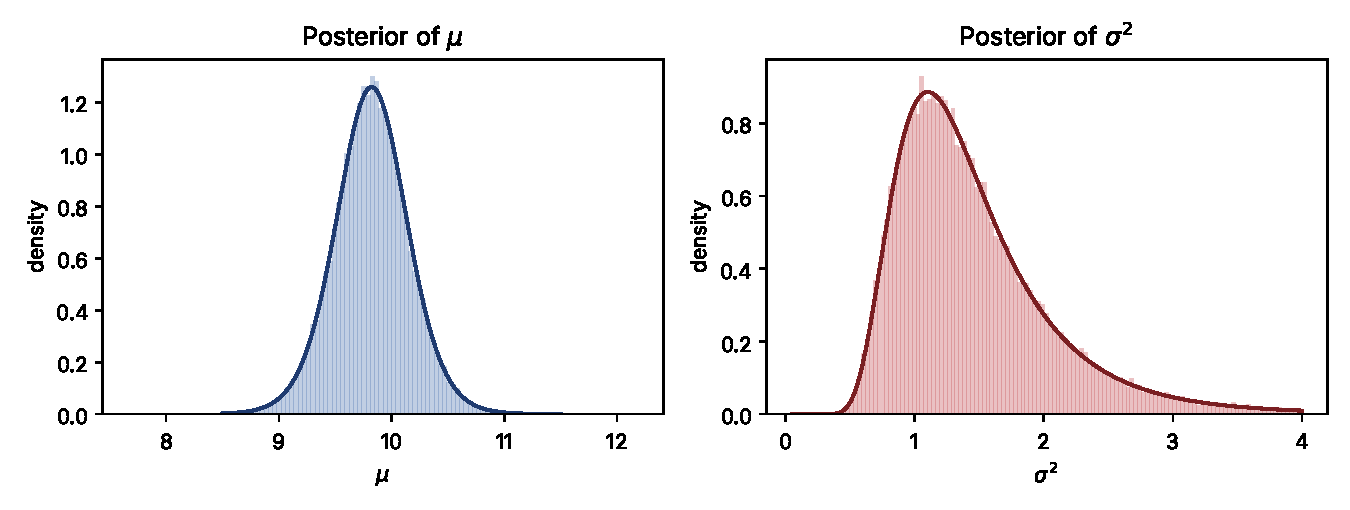
\includegraphics[width=0.9\linewidth]{q5_densities.pdf}\end{center}
{\small Histograms: 50{,}000 posterior draws. Curves: exact marginal densities.}

\textbf{(e)} Weak prior: $p_n=10.01$, $\mu_n=100.7/10.01=10.060$, $\nu_n=10.01$, and $SS_n=0.01+7.001+\frac{0.1}{10.01}(10.07)^2=8.024$.
\ans{\begin{tabular}{lcc}
 & Prior 1 ($\mu_0=9,p_0=3$) & Weak prior \\\midrule
$E[\mu\mid x]$ & 9.823 & 10.060 \\
95\% CI for $\mu$ & (9.155, 10.491) & (9.430, 10.690) \\
$P(\mu>10\mid x)$ & 0.289 & 0.582 \\
$E[\sigma^2\mid x]$ & 1.470 & 1.002 \\
95\% CI for $\sigma^2$ & (0.676, 3.135) & (0.392, 2.467)
\end{tabular}\\[4pt]
(Exact values; Monte Carlo estimates agree to about $\pm0.005$.)\\[4pt]
Under the weak prior the posterior of $\mu$ sits essentially at $\bar x=10.07$, as expected when $p_0\approx0$. The first prior pulls the mean down by about 0.24 toward $\mu_0=9$. With $p_0=3$ against $n=10$, the prior has weight $3/13\approx23\%$. The interval widths are similar (about 1.34 vs.\ 1.26), but the intervals are shifted, and $P(\mu>10\mid x)$ roughly doubles from 0.29 to 0.58. The first prior also inflates $\sigma^2$: its prior guess $SS_0/\nu_0=2$ exceeds the sample variance $7.001/9\approx0.78$, and the prior--data conflict term adds 2.64 to $SS_n$.\\[3pt]
\textbf{Conclusion:} with only $n=10$ observations, the data are not strong enough to wash out the informative prior. Point estimates are in the same neighborhood, but conclusions such as $P(\mu>10)$ are clearly prior-sensitive. A prior worth 3 observations is substantial relative to 10. With much larger $n$ the two analyses would converge.}

\end{document}
